\part{Fundamental electromagnetic principles and magnetic materials}
\title[Electromagnetic and material fundamentals]{Fundamental electromagnetic principles and magnetic materials}  
\date{}  
\frame{\titlepage} 

%%%%%%%%%%%%%%%%%%%%%%%%%%%%%%%%%%%%%%%%%%%%%%%%%%%%%%%%%%%%%
%% Ampere's circuital law: magnetic field strength %%
%%%%%%%%%%%%%%%%%%%%%%%%%%%%%%%%%%%%%%%%%%%%%%%%%%%%%%%%%%%%%
\begin{frame}
	\frametitle{Amp\`ere's circuital law: magnetic field strength}
	\begin{columns}
		\begin{column}{0.55\textwidth}
			Relates the circulation of a magnetic field around a closed loop to the electric current passing through the loop:
            \begin{align}
                \mbox{Integral form:} \quad &\oint_{\partial S} \bm{H} \cdot \mathrm{d}\bm{s} = I_{\mathrm{f}},\\
                \mbox{Differential form:} \quad &\nabla \times \bm{H} = \bm{J}_{\mathrm{f}}. 
            \end{align}
            Here, $\bm{H}$ is the magnetic field strength, $\bm{J}_{\mathrm{f}}$ is the free current density, and $I_{\mathrm{f}}$ is the free current enclosed by the loop $\partial S$. 
            \vspace{0.25cm}
            \begin{itemize}
                \item Free current: current that is not bound to a material (i.e., without polarization and magnetization currents).
                \item SI-unit: $[H] = \si{\ampere\per\metre}$
            \end{itemize}
		\end{column}
        \hfill
		\begin{column}{0.4\textwidth}
			\begin{figure}
				\centering
				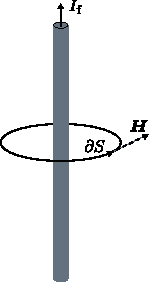
\includegraphics[height=0.7\textheight]{fig/lec02/Magnetic_field_strength_simple_conductor.pdf}
				\caption{Illustration of the magnetic field strength $\bm{H}$ around a simple conductor}
			\end{figure}
		\end{column}
		\end{columns}
\end{frame}

%%%%%%%%%%%%%%%%%%%%%%%%%%%%%%%%%%%%%%%%%%%%%%%%%%%%%%%%%%%%%
%% Ampere's circuital law %%
%%%%%%%%%%%%%%%%%%%%%%%%%%%%%%%%%%%%%%%%%%%%%%%%%%%%%%%%%%%%%
\begin{frame}
	\frametitle{Amp\`ere's circuital law: magnetic field strength example}
	\begin{columns}
		\begin{column}{0.55\textwidth}
			What is the free current $I_{\mathrm{f}}$ enclosed by the loop $\partial S$?
            \begin{itemize}
                \item The current $I_1$ flows in the direction of the loop $\partial S$ (according to right-hand rule).
                \item The current $I_1$ must be counted $N$ times due to the $N$ turns of wire around the loop $\partial S$.
                \item The current $I_2$ flows in the opposite direction of the loop $\partial S$ (according to right-hand rule).
                \item Result:
            \end{itemize}
            \vspace{0.25cm}
            \begin{equation*}
                I_\mathrm{f} = N \cdot I_1 - I_2.
            \end{equation*}
		\end{column}
        \hfill
		\begin{column}{0.45\textwidth}
			\begin{figure}
				\centering
				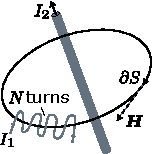
\includegraphics[height=0.5\textheight]{fig/lec02/Magnetic_field_strength_multiple_conductors.pdf}
				\caption{Arrangement with two electrical conductors}
			\end{figure}
		\end{column}
		\end{columns}
\end{frame}

%%%%%%%%%%%%%%%%%%%%%%%%%%%%%%%%%%%%%%%%%%%%%%%%%%%%%%%%%%%%%
%% Ampere's circuital law: magnetic flux %%
%%%%%%%%%%%%%%%%%%%%%%%%%%%%%%%%%%%%%%%%%%%%%%%%%%%%%%%%%%%%%
\begin{frame}
	\frametitle{Magnetic flux and flux linkage}
	\begin{columns}
		\begin{column}{0.575\textwidth}
			Variant for magnetic flux density $\bm{B}$:
            \begin{align}
                \mbox{Integral form:} \quad &\oint_{\partial S} \bm{B} \cdot \mathrm{d}\bm{l} = \mu_0 I,\\
                \mbox{Differential form:} \quad &\nabla \times \bm{B} = \mu_0\bm{J}. 
            \end{align}
            Here, $\mu_0$ is the permeability of free space, $\bm{J}$ is the total current density and $I$ is the total current enclosed by the loop $\partial S$. 
            \vspace{0.25cm}
            \begin{itemize}
                \item SI-unit: $[B] = \si{\tesla} = \si{\volt\second\per\metre\squared} = \si{\newton\per\ampere\per\metre}$
                \item Example contour $\partial S$  on the right covering $N$ turns and length $l$ (flux density within solenoid):
            \end{itemize}
            $$\oint_{\partial S} \bm{B} \cdot \mathrm{d}\bm{l} = N \mu_0 I  \Leftrightarrow B = \frac{N \mu_0 I}{l}$$
		\end{column}
        \hfill
		\begin{column}{0.425\textwidth}
            \vspace{-0.2cm}
			\begin{figure}
				\centering
				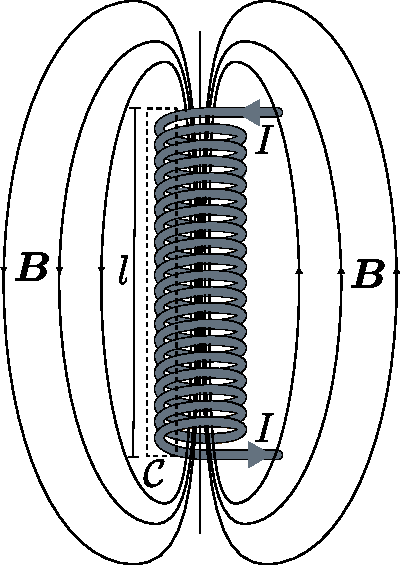
\includegraphics[height=0.68\textheight]{fig/lec02/Solenoid_Ampere_law.pdf}
				\caption{Magnetic flux $\Phi$ evaluated at the surface $\bm{S}$  (adapted from: \href{https://commons.wikimedia.org/wiki/File:Solenoid_and_Ampere_Law.png}{Wikimedia Commons}, Goodphy, \href{https://creativecommons.org/licenses/by-sa/4.0/deed.en}{CC BY-SA 4.0})}
			\end{figure}
		\end{column}
		\end{columns}
\end{frame}

%%%%%%%%%%%%%%%%%%%%%%%%%%%%%%%%%%%%%%%%%%%%%%%%%%%%%%%%%%%%%
%% Ampere's circuital law: magnetic flux %%
%%%%%%%%%%%%%%%%%%%%%%%%%%%%%%%%%%%%%%%%%%%%%%%%%%%%%%%%%%%%%
\begin{frame}
	\frametitle{Magnetic flux and flux linkage}
	\begin{columns}
		\begin{column}{0.575\textwidth}
			The magnetic flux $\Phi$ is the surface integral of the normal component of $\bm{B}$ over that surface:
            \begin{align}
                \Phi = \int_{S} \bm{B} \cdot \mathrm{d}\bm{S}. 
            \end{align}
            As there are no magnetic monopoles, the magnetic flux through a closed surface (which is covering a volume without holes) is always zero:
            \begin{align}
                \oint_{S} \bm{B} \cdot \mathrm{d}\bm{S} = 0.
            \end{align}
            The flux linkage $\Psi$ is the product of the magnetic flux $\Phi$ and the number of turns $N$ of a coil:
            \begin{align}
                \Psi = N  \Phi.
            \end{align}
		\end{column}
        \hfill
		\begin{column}{0.425\textwidth}
            \vspace{-0.2cm}
			\begin{figure}
				\centering
				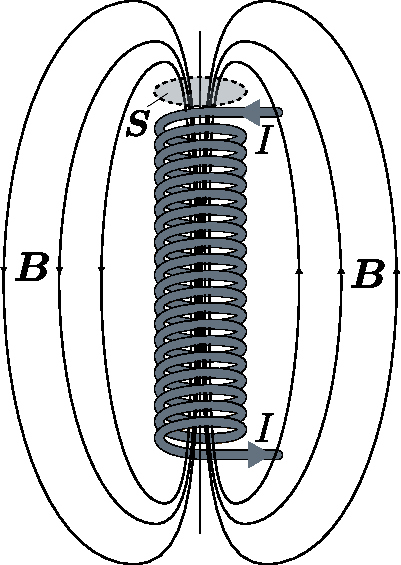
\includegraphics[height=0.68\textheight]{fig/lec02/Solenoid_Flux.pdf}
				\caption{Magnetic flux $\Phi$ evaluated at the surface $\bm{S}$  (adapted from: \href{https://commons.wikimedia.org/wiki/File:Solenoid_and_Ampere_Law.png}{Wikimedia Commons}, Goodphy, \href{https://creativecommons.org/licenses/by-sa/4.0/deed.en}{CC BY-SA 4.0})}
			\end{figure}
		\end{column}
		\end{columns}
\end{frame}

%%%%%%%%%%%%%%%%%%%%%%%%%%%%%%%%%%%%%%%%%%%%%%%%%%%%%%%%%%%%%
%% Boosting the magnet field with ferromagnetic materials %%
%%%%%%%%%%%%%%%%%%%%%%%%%%%%%%%%%%%%%%%%%%%%%%%%%%%%%%%%%%%%%
\begin{frame}
	\frametitle{Boosting the magnet field with ferromagnetic materials}
	\begin{columns}
		\begin{column}{0.575\textwidth}
			While $\bm{H}$ depends on the free currents applied to an object, $\bm{B}$ depends on the material properties of the object. In free space (vacuum), the relation is linear and represented by the magnetic constant $\mu_0$:
            \begin{align}
                \bm{B} = \mu_0 \bm{H} \quad \mbox{with} \quad \mu_0 \approx \SI{4 \pi e-7}{\newton\per\ampere\squared}.
            \end{align}
            To boost $\bm{B}$ for a given $\bm{H}$, ferromagnetic materials are typically used. These materials have a high relative magnetic permeability $\mu_{\mathrm{r}}$:
            \begin{align}
                \bm{B} = \mu \bm{H} = \mu_0 \mu_{\mathrm{r}} \bm{H}.
                \label{eq:linear_permeability} 
            \end{align}
            Note that $\mu_{\mathrm{r}}$ is a dimensionless quantity and that \eqref{eq:linear_permeability} assumes linear and isotropic material behavior.
		\end{column}
        \hfill
		\begin{column}{0.425\textwidth}
            \vspace{-0.2cm}
			\begin{figure}
				\centering
				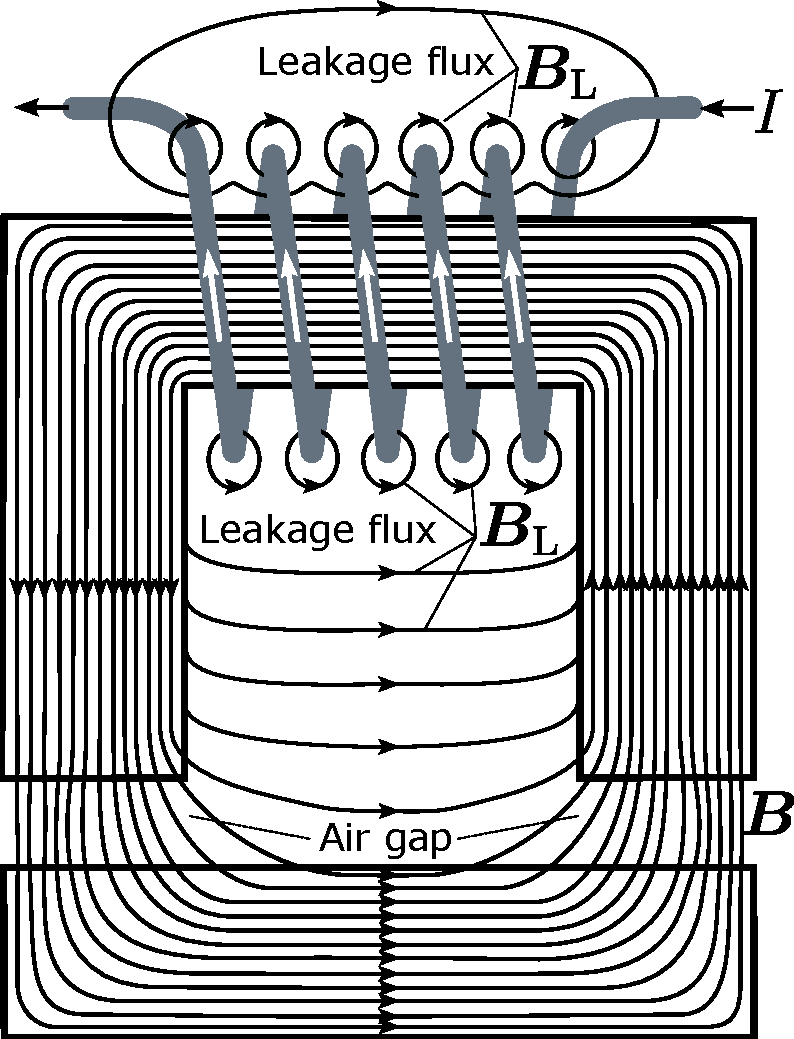
\includegraphics[height=0.68\textheight]{fig/lec02/Electromagnet_with_gap.pdf}
				\caption{Simplified magnetic field lines of an iron yoke with a coil  (adapted from: \href{https://en.m.wikipedia.org/wiki/File:Electromagnet_with_gap.svg}{Wikimedia Commons}, public domain)}
			\end{figure}
		\end{column}
		\end{columns}
\end{frame}

%%%%%%%%%%%%%%%%%%%%%%%%%%%%%%%%%%%%%%%%%%%%%%%%%%%%%%%%%%%%%
%% Relative permeability and magnetic saturation %%
%%%%%%%%%%%%%%%%%%%%%%%%%%%%%%%%%%%%%%%%%%%%%%%%%%%%%%%%%%%%%
\begin{frame}
	\frametitle{Relative permeability and magnetic saturation}
	\begin{columns}
		\begin{column}{0.575\textwidth}
			\begin{table}
            \centering
            \begin{tabular}{lc}
                \toprule
                Material & $\mu_{\mathrm{r}}$ (range)\\
                \midrule
                Air / copper / aluminum & $(\approx)$1 \\ 
                Iron (99.8\,\% pure) & 5000\\
                Electrical steel & 2000 - 35000\\
                Ferrite & 200 - 20000\\
                \bottomrule
            \end{tabular}
            \caption{Typical relative permeabilities of materials}
            \label{tab:rel_permeabilities}
            \end{table}
        Linear magnetic behavior ($\mu_{\mathrm{r}}=\mbox{const.}$) is only a local approximation. When considering larger $H$ ranges, the (differential) permeability becomes nonlinear:
        \begin{align}
            \mu_\mathrm{r}(H) =  \frac{\mathrm{d}B}{\mathrm{d}H}.
        \end{align}
		\end{column}
        \hfill
		\begin{column}{0.425\textwidth}
			\begin{figure}
				\centering
				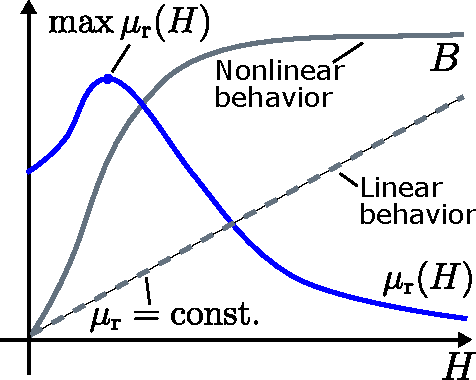
\includegraphics[height=0.5\textheight]{fig/lec02/Permeability_of_ferromagnet.pdf}
				\caption{Illustrative magnetisation curves for ferromagnets (and ferrimagnets) and corresponding permeabilities  (adapted from: \href{https://commons.wikimedia.org/wiki/File:Permeability_of_ferromagnet_by_Zureks.svg}{Wikimedia Commons}, public domain)}
			\end{figure}
		\end{column}
		\end{columns}
\end{frame}


%%%%%%%%%%%%%%%%%%%%%%%%%%%%%%%%%%%%%%%%%%%%%%%%%%%%%%%%%%%%%
%% Magnetic domains (1) %%
%%%%%%%%%%%%%%%%%%%%%%%%%%%%%%%%%%%%%%%%%%%%%%%%%%%%%%%%%%%%%
\begin{frame}
	\frametitle{Magnetic domains (1)}
    \begin{columns}
	\begin{column}{0.48\textwidth}
    \begin{itemize}
        \item Magnetic domains are regions within a material where the magnetic moments of atoms are aligned (``mini magnets'').
        \item The magnetization within each domain points in a uniform direction, but the magnetization of different domains may point in different directions.
    \end{itemize}
    \end{column}
    \hfill
    \begin{column}{0.52\textwidth}
        \begin{figure}
            \centering
            \movie{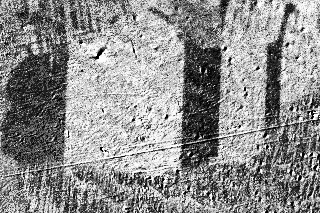
\includegraphics[height=0.3\textheight]{fig/lec02/Moving_magnetic_domains_preview.png}}{fig/lec02/Moving_magnetic_domains.gif}
            \caption{Animation of moving domain walls (source: \href{https://commons.wikimedia.org/wiki/File:Moving_magnetic_domains_by_Zureks.gif}{Wikimedia Commons}, Zureks, \href{https://creativecommons.org/licenses/by-sa/3.0/deed.en}{CC BY-SA 3.0})}
        \end{figure}
    \end{column}
\end{columns}
\begin{figure}
\begin{columns}
	\begin{column}{0.6\textwidth}
            \centering
            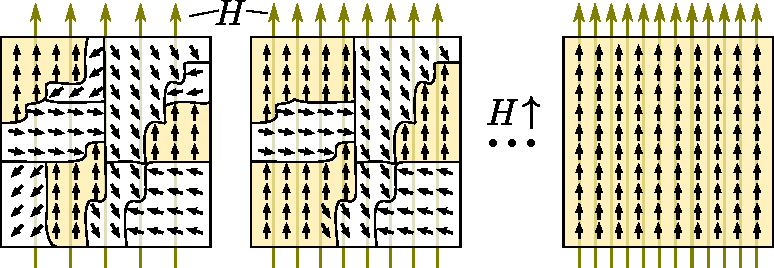
\includegraphics[width=0.9\textwidth]{fig/lec02/Growing-magnetic-domains.pdf}
    \end{column}
    \begin{column}{0.35\textwidth}
        \caption{\raggedright Change of magnetic domains due to an external magnetic field  (adapted from: \href{https://de.wikipedia.org/wiki/Datei:Growing-magnetic-domains.svg}{Wikimedia Commons}, M. Run, \href{https://creativecommons.org/licenses/by-sa/4.0/deed.en}{CC BY-SA 4.0})}
    \end{column}
\end{columns}
\end{figure}
\end{frame}

%%%%%%%%%%%%%%%%%%%%%%%%%%%%%%%%%%%%%%%%%%%%%%%%%%%%%%%%%%%%%
%% Magnetic domains (2) %%
%%%%%%%%%%%%%%%%%%%%%%%%%%%%%%%%%%%%%%%%%%%%%%%%%%%%%%%%%%%%%
\begin{frame}
	\frametitle{Magnetic domains (2)}
    \begin{itemize}
        \item A large region of material with a constant magnetization throughout creates a large magnetic field (diagram a) below). This requires a lot of magnetostatic energy stored in the field. 
        \item To reduce this energy, the sample can ``split'' into two domains, with the magnetization in opposite directions in each domain which reduces the overall field (diagram b) below).
        \item  To reduce the field energy further, each of these domains can split also, resulting in smaller parallel domains with magnetization in alternating directions, with smaller amounts of field outside the material (diagram c) below).
    \end{itemize}
\begin{figure}
\begin{columns}
	\begin{column}{0.55\textwidth}
            \centering
            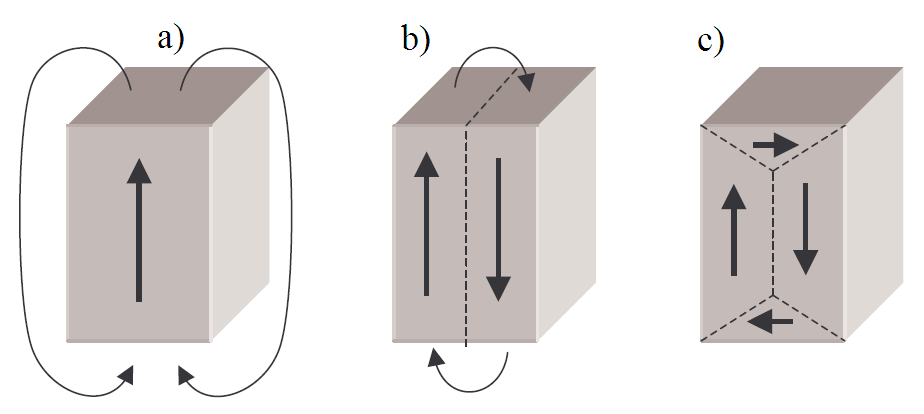
\includegraphics[width=0.8\textwidth]{fig/lec02/Magnetic_domains_energy_min.png}
    \end{column}
    \begin{column}{0.4\textwidth}
        \caption{\raggedright Simplified representation of the formation of magnetic domains on the basis of energy minimization  (source: \href{https://commons.wikimedia.org/wiki/File:Powstawanie_domen_by_Zureks.png}{Wikimedia Commons}, public domain)}
    \end{column}
\end{columns}
\end{figure}
\end{frame}

%%%%%%%%%%%%%%%%%%%%%%%%%%%%%%%%%%%%%%%%%%%%%%%%%%%%%%%%%%%%%
%% Hysteresis %%
%%%%%%%%%%%%%%%%%%%%%%%%%%%%%%%%%%%%%%%%%%%%%%%%%%%%%%%%%%%%%
\begin{frame}
	\frametitle{Hysteresis}
	\begin{columns}
		\begin{column}{0.575\textwidth}
            \begin{itemize}
                \item Material defects lead to small, random jumps in magnetization called Barkhausen jumps.
                \item Domain walls move irregularly.
                \item Process also depends on the history of the magnetization process (dynamic system).
            \end{itemize}
			\begin{figure}
                \centering
                \movie{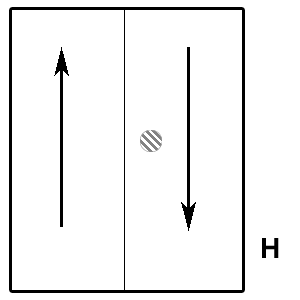
\includegraphics[height=0.3\textheight]{fig/lec02/Barkhausen_jump_preview.png}}{fig/lec02/Barkhausen_jump.gif}
                \caption{Animation of the Barkhausen jump (source: \href{https://commons.wikimedia.org/wiki/File:Barkhausensprung.gif}{Wikimedia Commons},  public domain)}
            \end{figure}
		\end{column}
        \hfill
		\begin{column}{0.425\textwidth}
            \vspace{-0.2cm}
			\begin{figure}
				\centering
				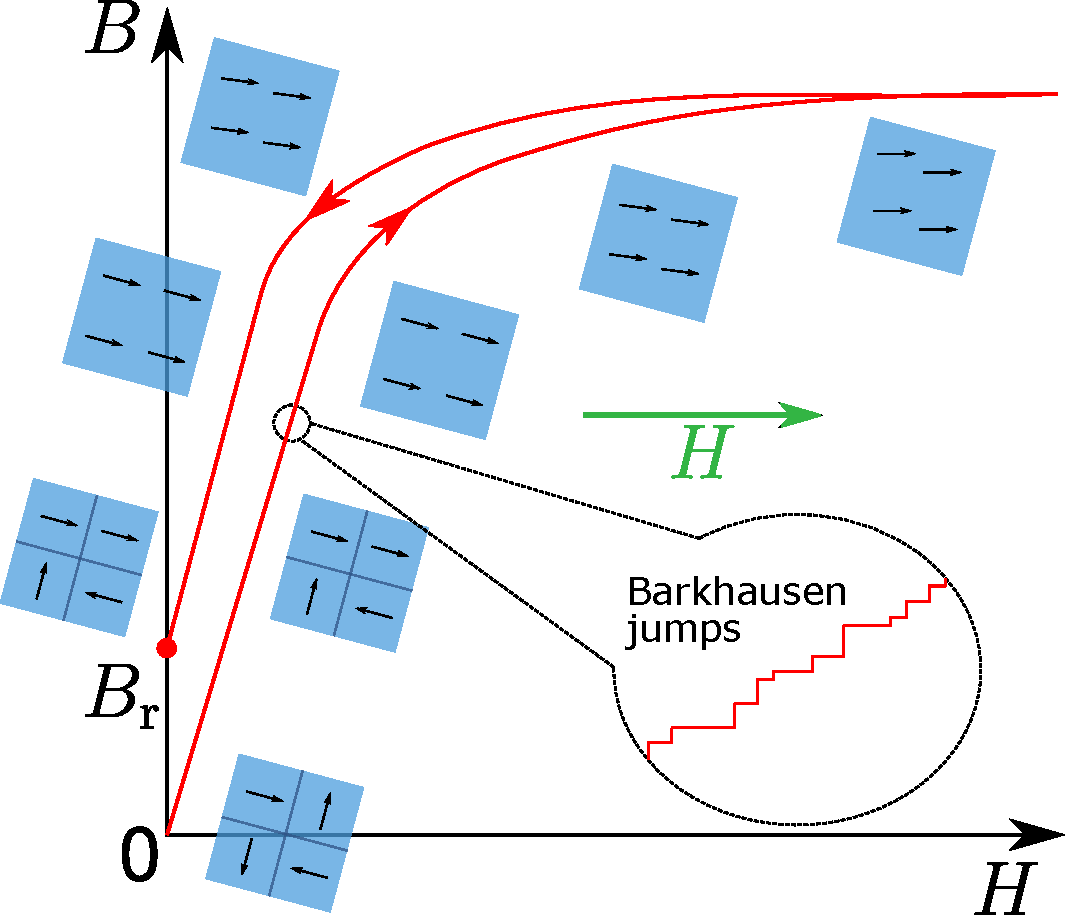
\includegraphics[height=0.5\textheight]{fig/lec02/Ferromagnet_magnetization_and_magnetic_domains_and_hysteresis.pdf}
				\caption{Simplified hysteresis curve in first quadrant with magnetic domains illustration (adapted from: \href{https://commons.wikimedia.org/wiki/File:Ferromagnet_magnetization_and_magnetic_domains_and_hysteresis.svg}{Wikimedia Commons}, Fralama, \href{https://creativecommons.org/licenses/by-sa/3.0/deed.enn}{CC BY-SA 3.0})}
			\end{figure}
		\end{column}
		\end{columns}
\end{frame}

%%%%%%%%%%%%%%%%%%%%%%%%%%%%%%%%%%%%%%%%%%%%%%%%%%%%%%%%%%%%%
%% Hysteresis curve and losses %%
%%%%%%%%%%%%%%%%%%%%%%%%%%%%%%%%%%%%%%%%%%%%%%%%%%%%%%%%%%%%%
\begin{frame}
	\frametitle{Hysteresis curve and losses}
	\begin{columns}
		\begin{column}{0.5\textwidth}
            \begin{itemize}
                \item With an external and varying field $H$, a closed hysteresis curve is obtained.
                \item Traversing through the curve requires to move the domain walls and rotate the elementary magnets within the domains.
                \item This process requires work and leads to heat dissipation (losses).
                \item The area enclosed by the hysteresis curve is identical to the relative remagnetization work (per volume, that is, $[w_{\mathrm{h}}]=\si{\joule\per\metre\cubed}$):
            \end{itemize}
            \begin{align}
                w_{\mathrm{h}} = \oint \bm{H} \cdot \mathrm{d}\bm{B}.
            \end{align}
		\end{column}
        \hfill
		\begin{column}{0.475\textwidth}
            \vspace{-0.2cm}
			\begin{figure}
				\centering
				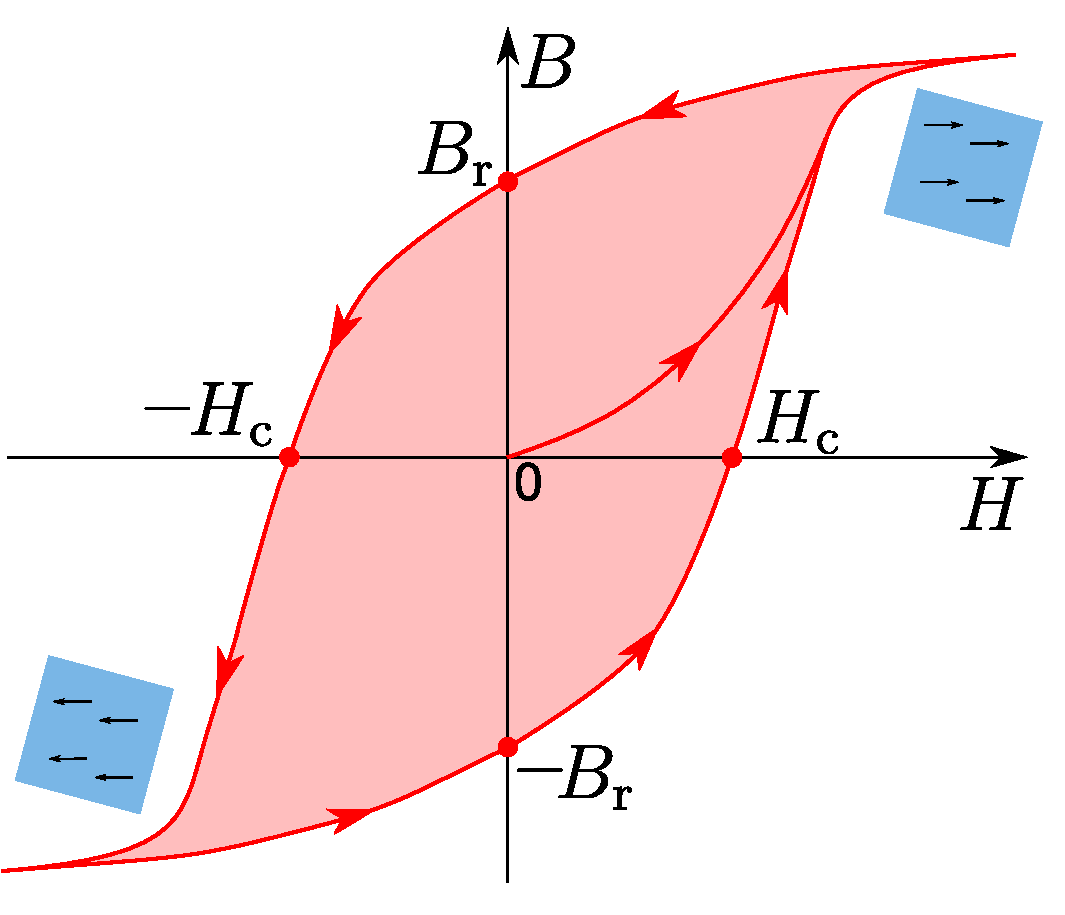
\includegraphics[height=0.55\textheight]{fig/lec02/Hyteresis_curve_full.pdf}
				\caption{Exemplary hysteresis curve with $B_\mathrm{r}$ being the remanence field density and $H_\mathrm{c}$ the coercivity field strength}
			\end{figure}
		\end{column}
		\end{columns}
\end{frame}

%%%%%%%%%%%%%%%%%%%%%%%%%%%%%%%%%%%%%%%%%%%%%%%%%%%%%%%%%%%%%
%% How can we model the hysteresis losses? %%
%%%%%%%%%%%%%%%%%%%%%%%%%%%%%%%%%%%%%%%%%%%%%%%%%%%%%%%%%%%%%
\begin{frame}
	\frametitle{How can we model the hysteresis losses?}
	\begin{columns}
		\begin{column}{0.5\textwidth}
            \vspace{-0.15cm}
            \begin{enumerate}
                \item \textbf{Data look-up table:} Measure the hysteresis curve and its losses directly on a test bench (cf. \href{https://www.princeton.edu/~minjie/magnet.html}{MagNet project data hub}).
                \item \textbf{Loss-fitted models:} Use empirical models to fit the hysteresis losses (e.g., Steinmetz model):
                $$P_{\mathrm{h}} = kf^a \max\{B\}^b.$$
                \item \textbf{Curve-fitted models:} Use empirical models to describe the hysteresis curve and derive the losses (e.g., ODE as in the Jiles-Atherton model):
                $$\frac{\mathrm{d}B}{\mathrm{d}H} = f(B,H).$$
            \end{enumerate}
		\end{column}
        \hfill
		\begin{column}{0.475\textwidth}
            \vspace{-0.2cm}
			\begin{figure}
				\centering
				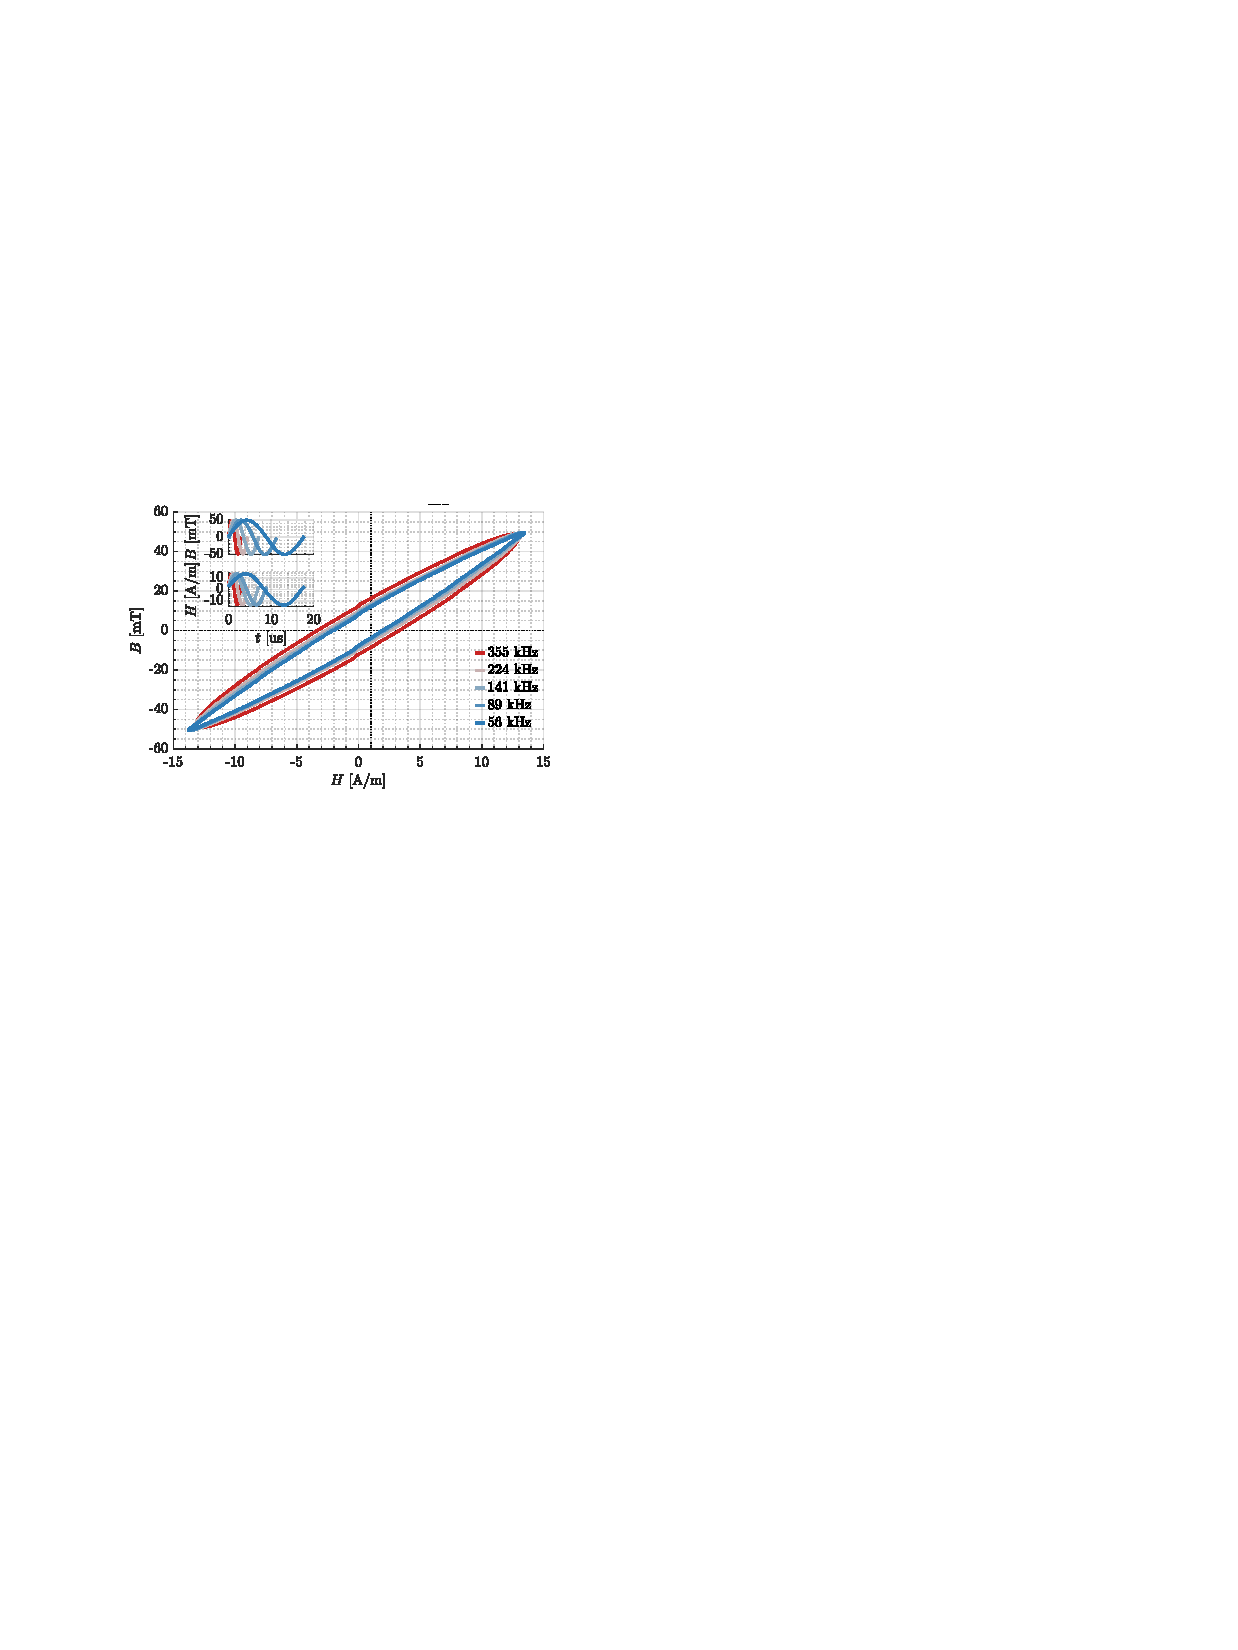
\includegraphics[height=0.55\textheight]{fig/lec02/Hysteresis_curve_Serrano_et_al.pdf}
				\caption{Measured $B$-$H$ loops for sinusoidal excitation at different frequencies (source: \href{https://ieeexplore.ieee.org/abstract/document/10169101}{IEEE TPEL}, Serrano et al., \href{https://creativecommons.org/licenses/by/4.0/}{CC BY 4.0})}
			\end{figure}
		\end{column}
		\end{columns}
\end{frame}

%%%%%%%%%%%%%%%%%%%%%%%%%%%%%%%%%%%%%%%%%%%%%%%%%%%%%%%%%%%%%
%% Alternative to boost the magnet field: permanent magnets %%
%%%%%%%%%%%%%%%%%%%%%%%%%%%%%%%%%%%%%%%%%%%%%%%%%%%%%%%%%%%%%
\begin{frame}
	\frametitle{Alternative to boost the magnet field: permanent magnets (PMs)}
    \begin{columns}
        \begin{column}{0.48\textwidth}
        \begin{itemize}
            \item Create own persistent magnetic fields.
            \item Consist of hard ferromagnetic (or ferrimagnetic) materials.
            \item Nearly constant magnetiziation offset $\bm{B}_\mathrm{PM}$ in the usual operating range:
            \begin{align}
                \bm{B} = \mu_0 \mu_{\mathrm{r}} \bm{H} \approx \mu_0 \bm{H} + \bm{B}_\mathrm{PM}.
            \end{align}
        \end{itemize}
        \end{column}
        \hfill
        \begin{column}{0.4\textwidth}
            \begin{figure}
                \centering
                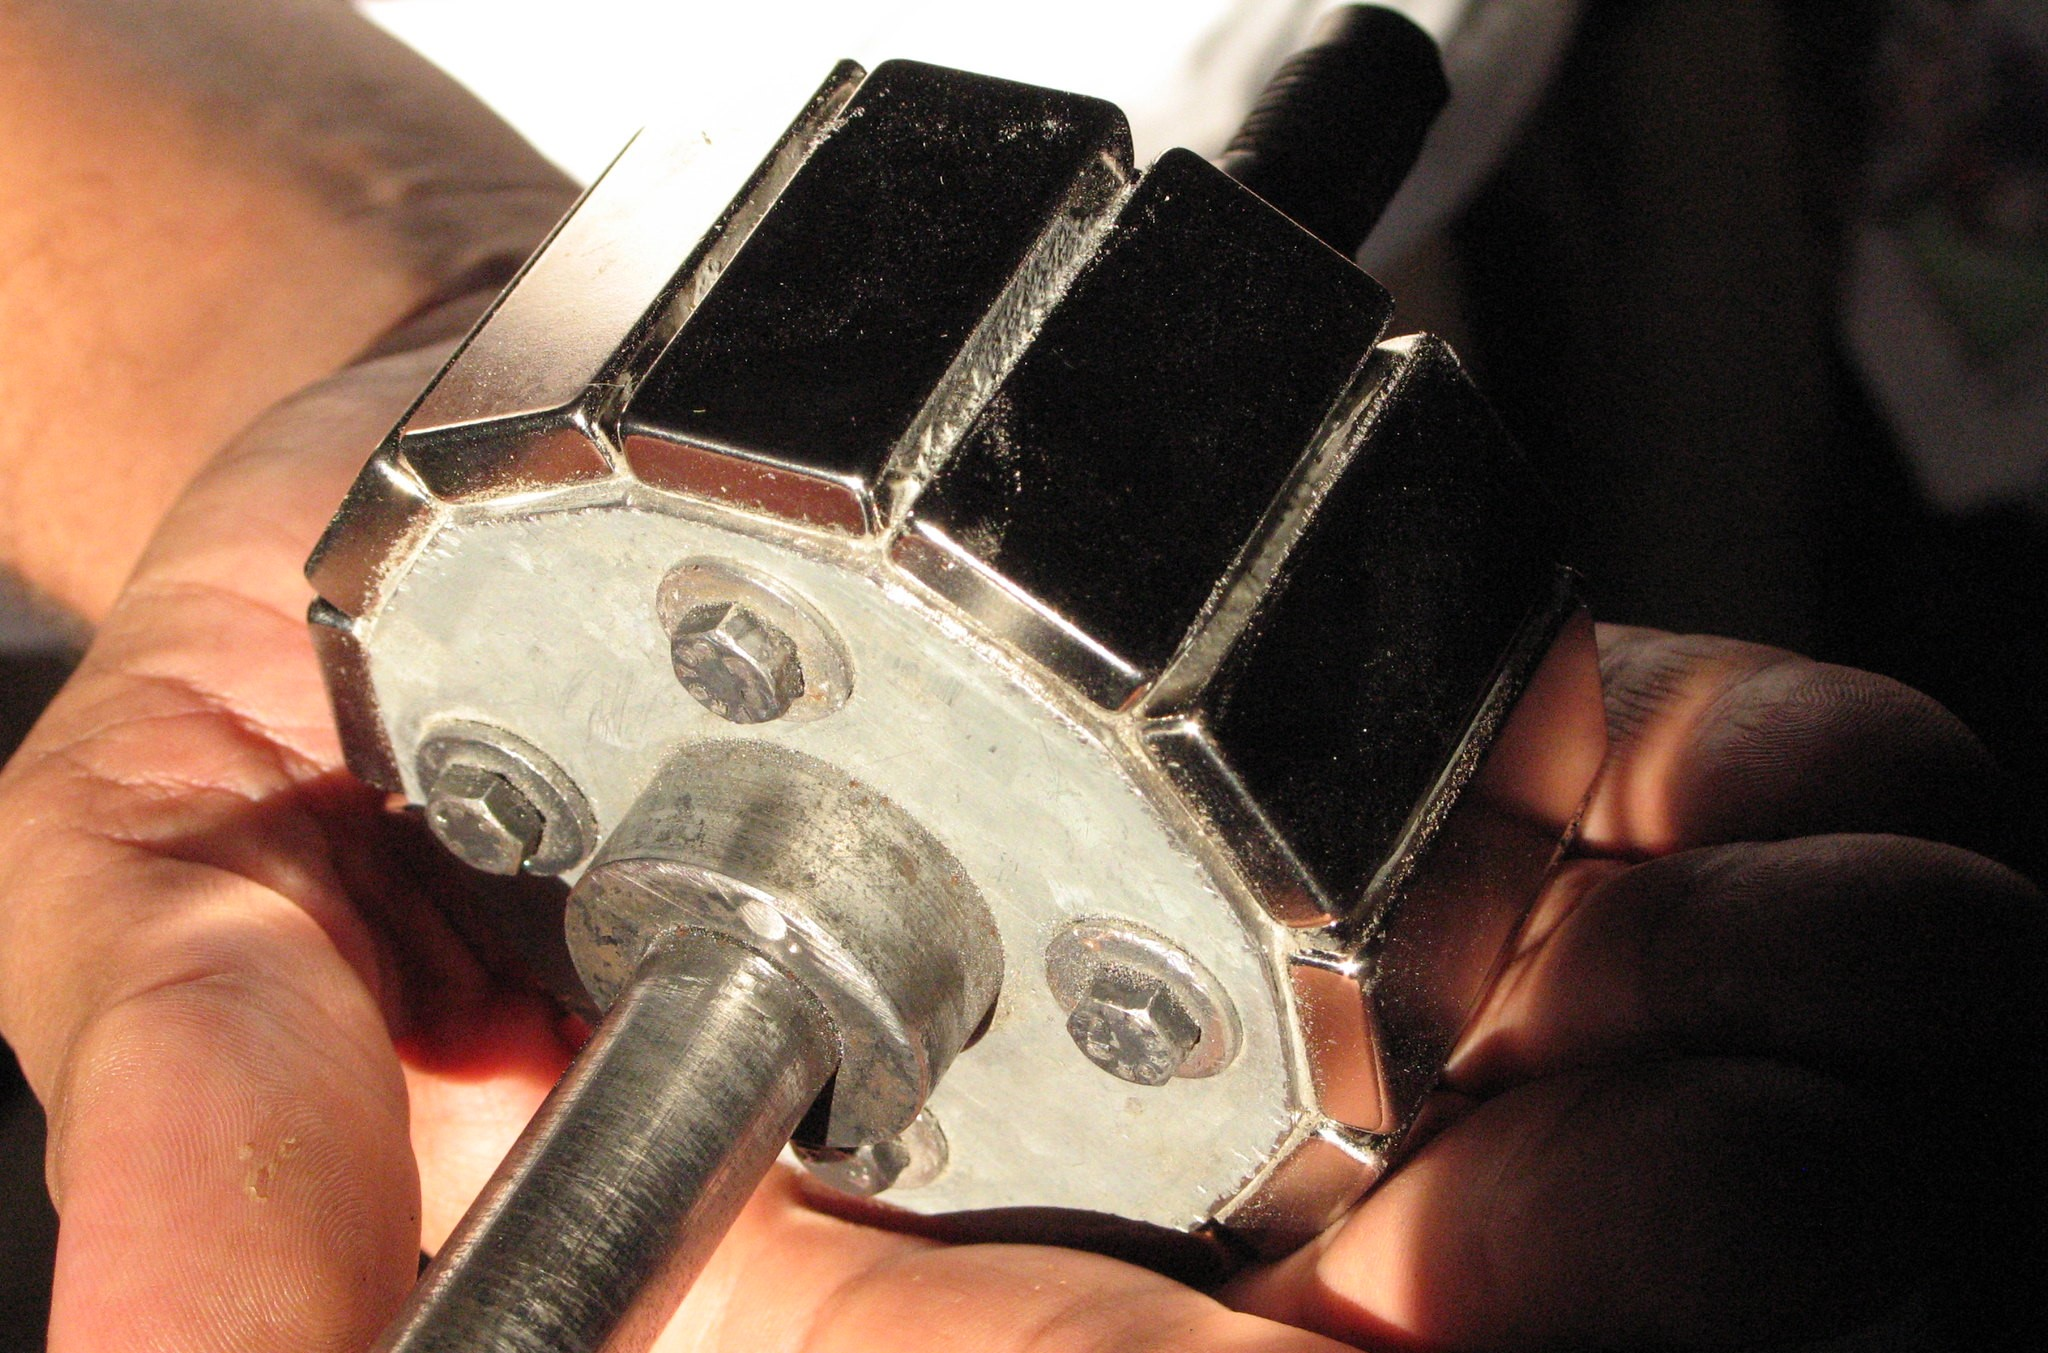
\includegraphics[width=0.65\textwidth]{fig/lec02/PM_rotor_example.jpg}
                \caption{PMs on a rotor (source: \href{https://www.flickr.com/photos/aidg/2382339376}{flickr.com}, AIDG, \href{https://creativecommons.org/licenses/by-nc-sa/2.0/}{CC BY-NC-SA 2.0})}
            \end{figure}
        \end{column}
    \end{columns}
    \begin{figure}
    \begin{columns}
        \begin{column}{0.6\textwidth}
                \centering
                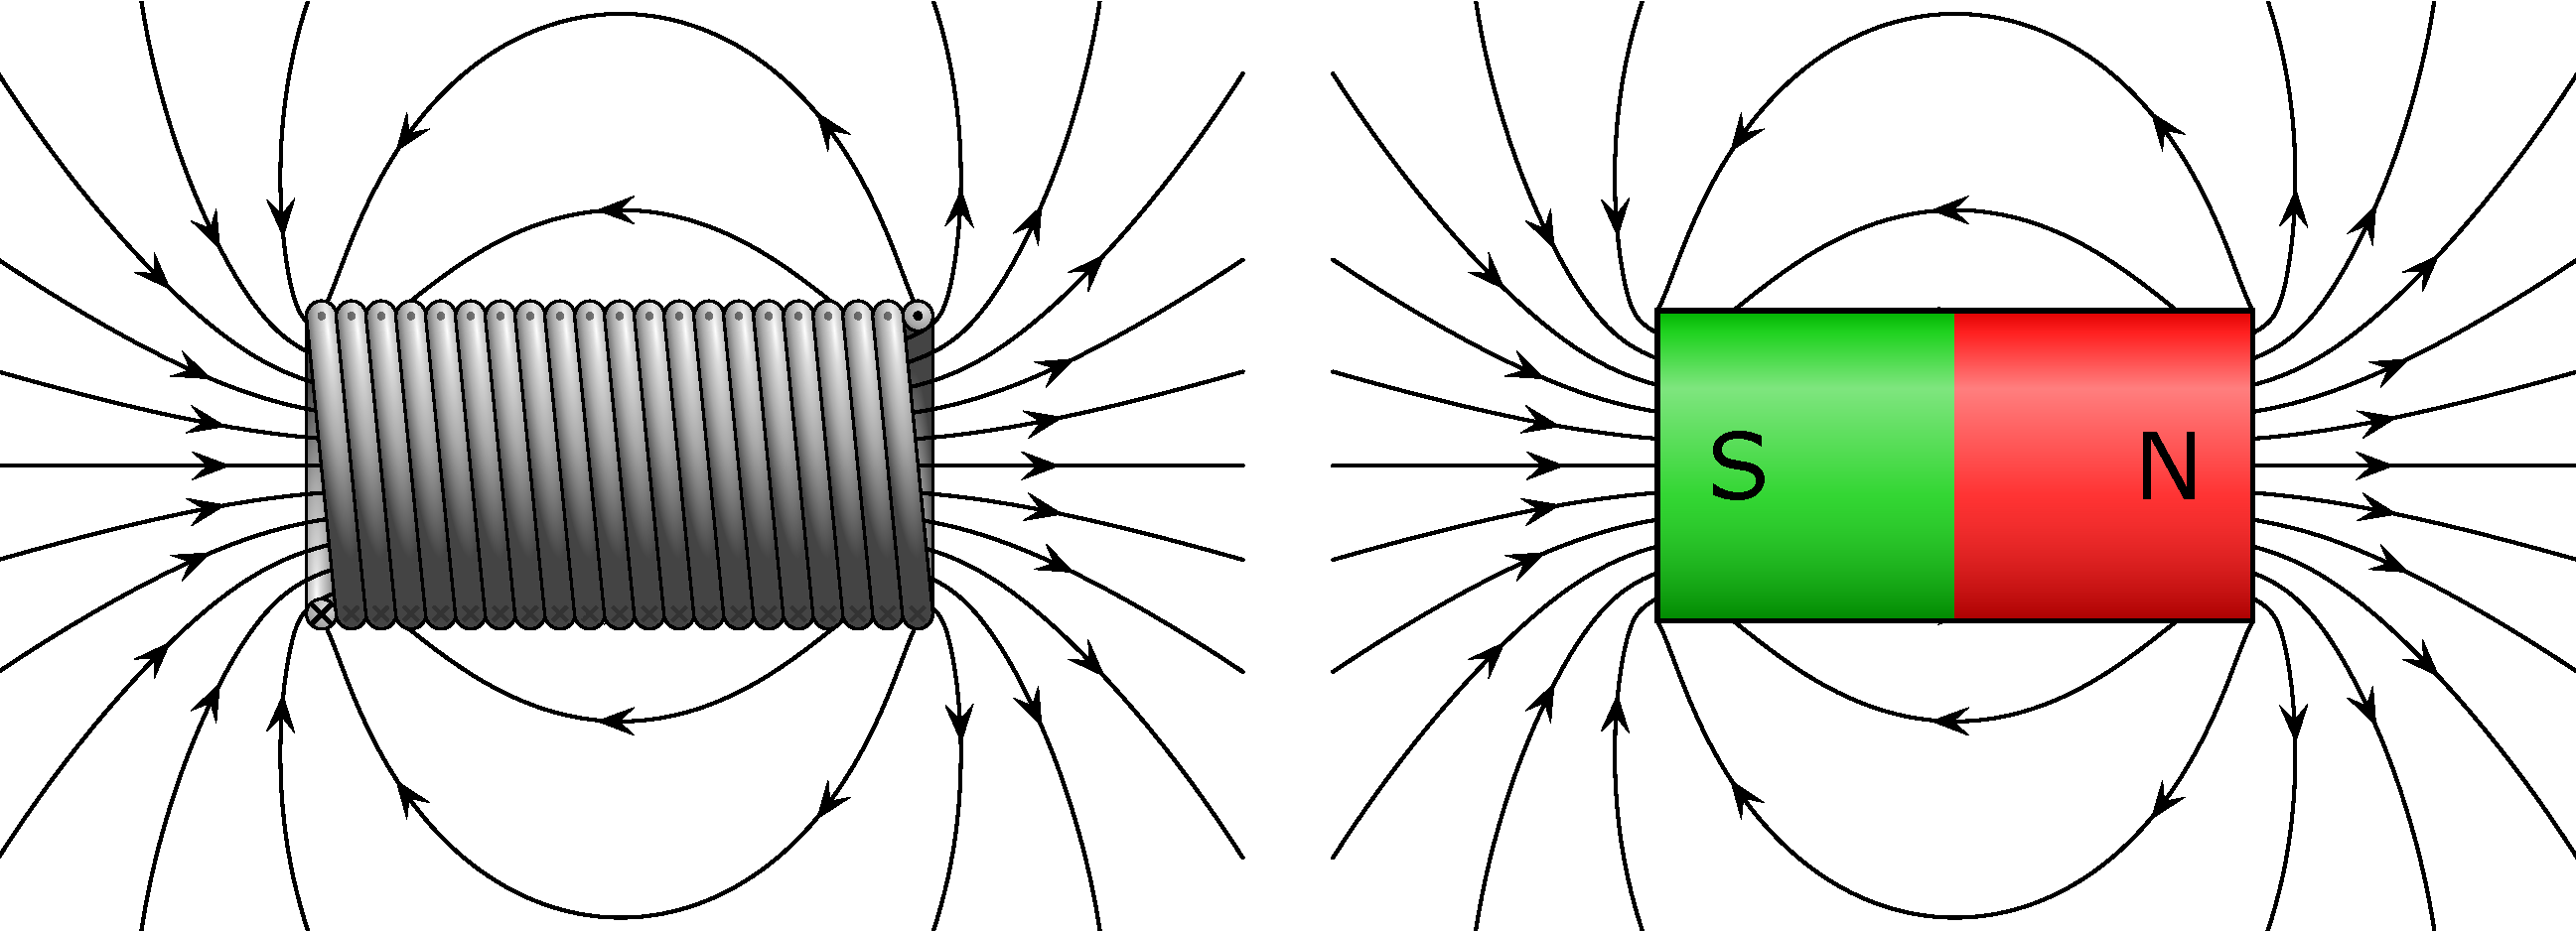
\includegraphics[width=0.9\textwidth]{fig/lec02/Coil_magnet_comparison.pdf}
        \end{column}
        \begin{column}{0.35\textwidth}
            \caption{\raggedright Permanent magnets as alternatives to current-based excitation  (source: \href{https://commons.wikimedia.org/wiki/File:VFPt_cylindrical_tightly-wound_coil-and-bar-magnet-comparison.svg}{Wikimedia Commons}, M. Run, \href{https://creativecommons.org/licenses/by-sa/3.0/deed.en}{CC BY-SA 3.0})}
        \end{column}
    \end{columns}
    \end{figure}
    \end{frame}

%%%%%%%%%%%%%%%%%%%%%%%%%%%%%%%%%%%%%%%%%%%%%%%%%%%%%%%%%%%%%
%% Hyteresis curve of permanent magnets %%
%%%%%%%%%%%%%%%%%%%%%%%%%%%%%%%%%%%%%%%%%%%%%%%%%%%%%%%%%%%%%
\begin{frame}
	\frametitle{Hyteresis curve of permanent magnets}
	\begin{columns}
		\begin{column}{0.45\textwidth}
            \begin{itemize}
                \item PM's magnetization is nearly  completely saturated and constant in common operation area.
                \item The greater the coercivity $H_\mathrm{c}$, the greater the resistance of the PM to demagnetization by external fields.
                \item Beyond the so-called knee point, PMs are (partially) demagnetized.
                \item Important figure of merit is the so called energy product:
                \begin{align}
                    (BH)_{\max} = \max \left\{- B H \right\}.
                \end{align}
                \item The higher $(BH)_{\max}$ the less PM material is needed for an application.
            \end{itemize}
		\end{column}
        \hfill
		\begin{column}{0.42\textwidth}
            \vspace{-0.2cm}
			\begin{figure}
				\centering
				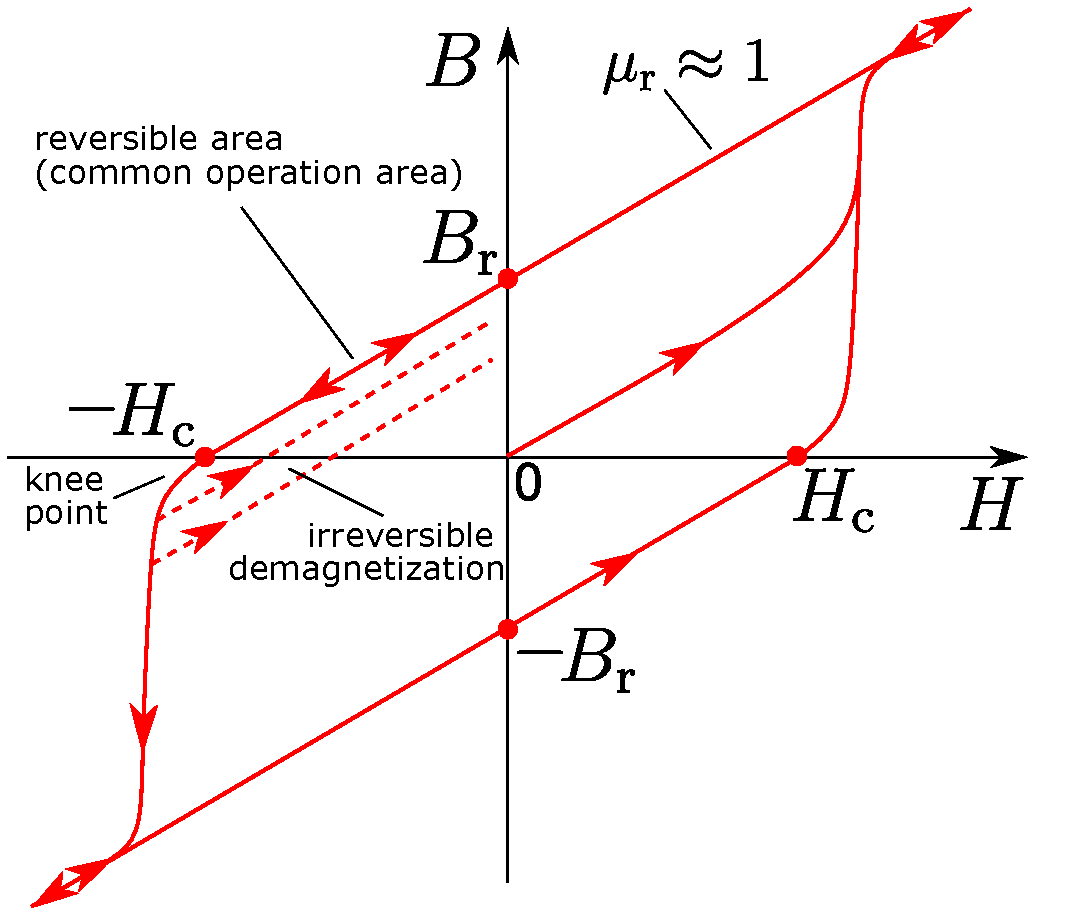
\includegraphics[height=0.6\textheight]{fig/lec02/Hyteresis_curve_PM.pdf}
				\caption{Exemplary hysteresis curve of a permanent magnet}
			\end{figure}
		\end{column}
		\end{columns}
\end{frame}

%%%%%%%%%%%%%%%%%%%%%%%%%%%%%%%%%%%%%%%%%%%%%%%%%%%%%%%%%%%%%
%% Hyteresis curve of permanent magnets (temperature dependence) %%
%%%%%%%%%%%%%%%%%%%%%%%%%%%%%%%%%%%%%%%%%%%%%%%%%%%%%%%%%%%%%
\begin{frame}
	\frametitle{Hyteresis curve of permanent magnets (temperature dependence)}
	\begin{columns}
		\begin{column}{0.4\textwidth}
            \begin{itemize}
                \item Besides pressure and vibrations, PMs are also sensitive to temperature.
                \item The coercivity $H_\mathrm{c}$ and the remanence $B_\mathrm{r}$ decrease with increasing temperature.
                \item Hence, with higher temperatures, a PM gets more susceptible to demagnetization.
            \end{itemize}
		\end{column}
        \hspace{0.25cm}
		\begin{column}{0.4\textwidth}
			\begin{figure}
				\centering
				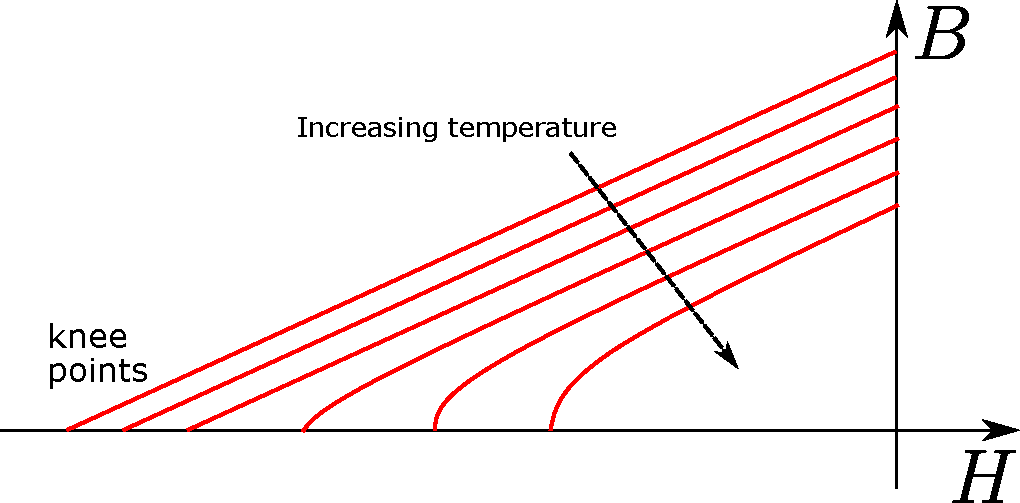
\includegraphics[height=0.4\textheight]{fig/lec02/Hyteresis_curve_PM_temperature.pdf}
				\caption{Qualitative representation of the temperature dependence of permanent magnets}
			\end{figure}
		\end{column}
		\end{columns}
\end{frame}

%%%%%%%%%%%%%%%%%%%%%%%%%%%%%%%%%%%%%%%%%%%%%%%%%%%%%%%%%%%%%
%% Energy product overview of permanent magnets %%
%%%%%%%%%%%%%%%%%%%%%%%%%%%%%%%%%%%%%%%%%%%%%%%%%%%%%%%%%%%%%
\begin{frame}
	\frametitle{Energy product overview of permanent magnets}
        \begin{figure}
            \centering
            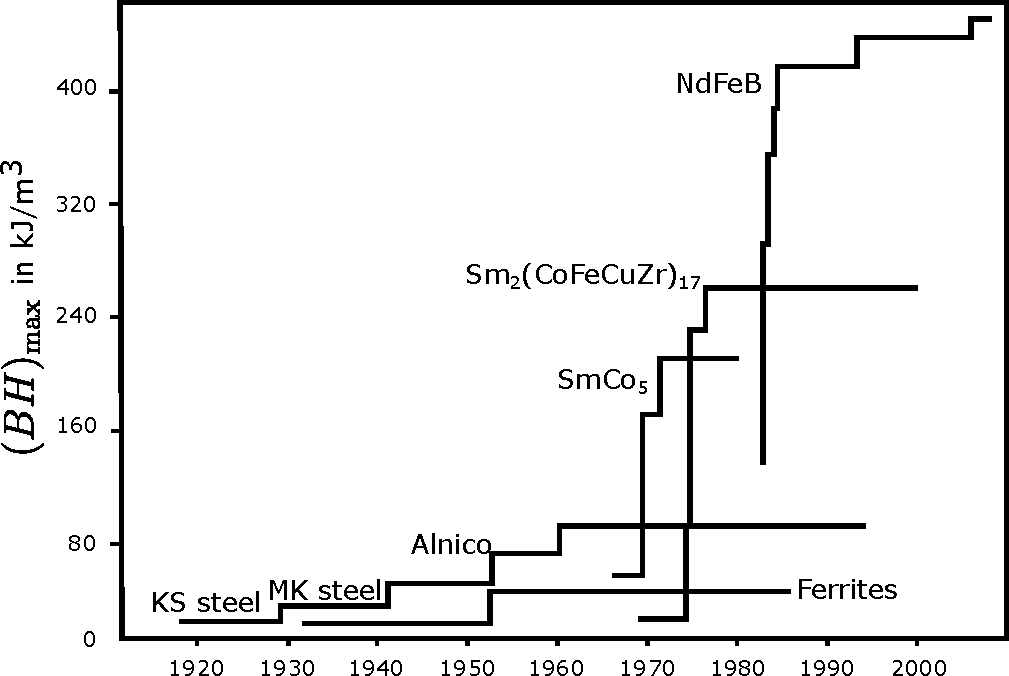
\includegraphics[height=0.65\textheight]{fig/lec02/PM_energy_product.pdf}
            \caption{Historic development of PM materials and their energy product (source: \href{https://commons.wikimedia.org/wiki/File:Magnetische_Energiedichte.svg}{Wikimedia Commons}, Kopiersperre, \href{https://creativecommons.org/licenses/by-sa/4.0/deed.en}{CC BY-SA 4.0})}
        \end{figure}
\end{frame}


%%%%%%%%%%%%%%%%%%%%%%%%%%%%%%%%%%%%%%%%%%%%%%%%%%%%%%%%%%%%%
%% Manufacturing process of NdFeB permanent magnets %%
%%%%%%%%%%%%%%%%%%%%%%%%%%%%%%%%%%%%%%%%%%%%%%%%%%%%%%%%%%%%%
\begin{frame}
	\frametitle{Manufacturing process of NdFeB permanent magnets}
        \begin{figure}
            \centering
            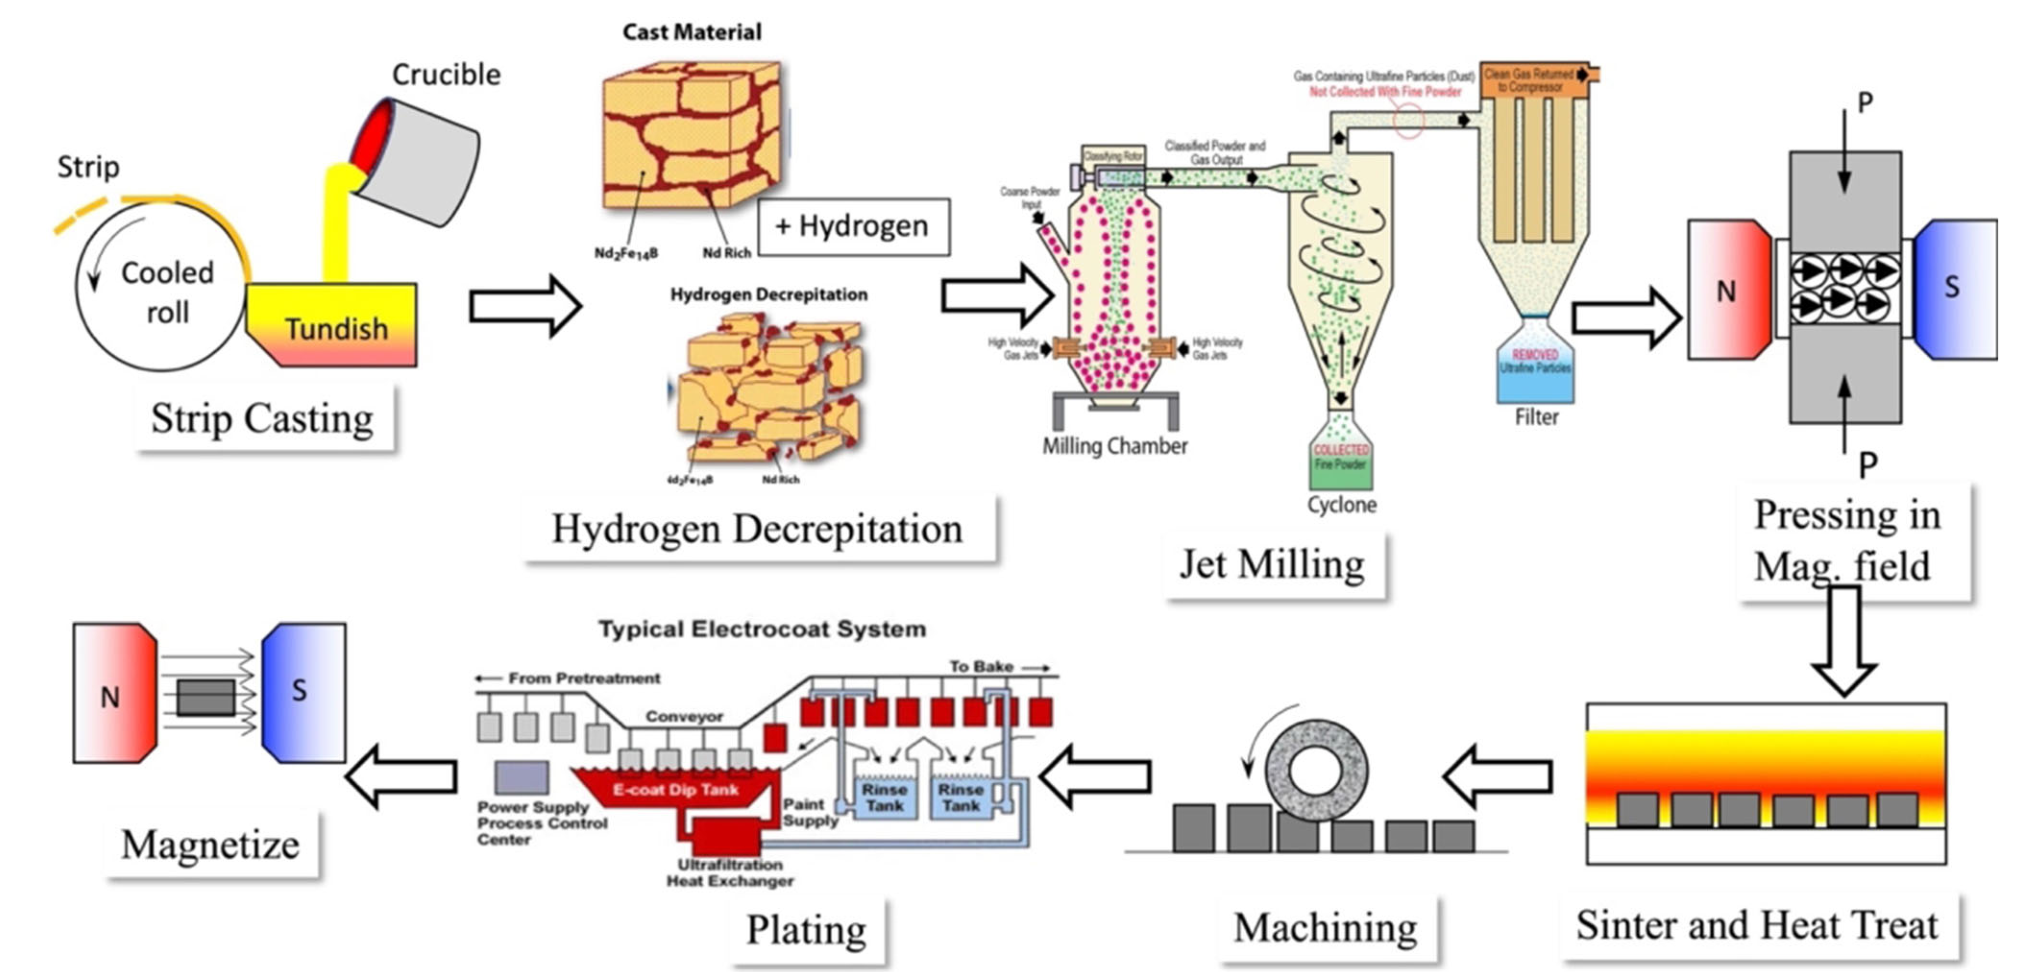
\includegraphics[height=0.65\textheight]{fig/lec02/Production_process_NdFeB_magnets.png}
            \caption{Basic process steps for the NdFeB-based magnets (source: \href{https://link.springer.com/article/10.1007/S11837-022-05156-9}{Springer JOM}, J. Cui et al., \href{https://creativecommons.org/licenses/by/4.0/}{CC BY 4.0})}
        \end{figure}
\end{frame}

%%%%%%%%%%%%%%%%%%%%%%%%%%%%%%%%%%%%%%%%%%%%%%%%%%%%%%%%%%%%%
%% Electromagnetic induction %%
%%%%%%%%%%%%%%%%%%%%%%%%%%%%%%%%%%%%%%%%%%%%%%%%%%%%%%%%%%%%%
\begin{frame}
	\frametitle{Electromagnetic induction}
    \begin{columns}
		\begin{column}{0.6\textwidth}
            A changing magnetic field induces an electric field according to the Maxwell–Faraday equation:
            \begin{align}
                \mbox{Integral form:} \quad & \oint_{\partial S} \bm{E} \cdot \mathrm{d}\bm{s} = -\int_{S}\frac{\partial \bm{B}}{\partial t}\cdot\mathrm{d}\bm{S},\\
                \mbox{Differential form:} \quad &\nabla \times \bm{E} = -\frac{\partial \bm{B}}{\partial t}.
            \end{align}
            Here, $\bm{E}$ is the electric field strength and $\bm{S}$ is the surface enclosed by the loop $\partial\mathcal{S}$.
            \begin{itemize}
                \item Lentz's law: The induced electric field opposes the change in magnetic field (negative sign above).
                \item SI-unit: $[E] = \si{\volt\per\metre}$
            \end{itemize}
		\end{column}
        \hfill
		\begin{column}{0.38\textwidth}
			\begin{figure}
				\centering
				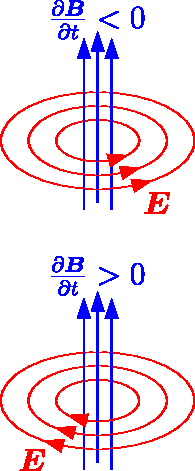
\includegraphics[height=0.6\textheight]{fig/lec02/Electromagnetic_induction.pdf}
				\caption{Representation of the magnetic and electric field relation (adapted from: \href{https://commons.wikimedia.org/wiki/File:Electromagnetic_induction.svg}{Wikimedia Commons}, Qniemiec, \href{https://creativecommons.org/licenses/by-sa/3.0/deed.en}{CC BY-SA 3.0})}
			\end{figure}
		\end{column}
		\end{columns}
\end{frame}

%%%%%%%%%%%%%%%%%%%%%%%%%%%%%%%%%%%%%%%%%%%%%%%%%%%%%%%%%%%%%
%% Electromotive force (EMF) and electromagnetic induction %%
%%%%%%%%%%%%%%%%%%%%%%%%%%%%%%%%%%%%%%%%%%%%%%%%%%%%%%%%%%%%%
\begin{frame}
	\frametitle{Electromotive force (EMF) and electromagnetic induction}
    \begin{columns}
		\begin{column}{0.55\textwidth}
            If the integration path $\partial S$ is identical to a conductor loop, the changing magnetic field induces a voltage $u_\mathrm{i}$ (electromotive force, EMF) according to Faraday's law:
            \begin{align*}
                u_\mathrm{i} =\oint_{\partial\mathcal{S}} \bm{E} \cdot \mathrm{d}\bm{s} = -\int_{S}\frac{\partial \bm{B}}{\partial t}\cdot\mathrm{d}\bm{S}.
            \end{align*}
        \begin{itemize}
            \item Despite its name, the term EMF does not describe a force in the physical sense (as $u_\mathrm{i}$ is obviously a voltage).
            \item The term remains a historical artifact from the early days of electrical engineering, but is still frequently used in today's literature. 
        \end{itemize}
		\end{column}
        \hfill
		\begin{column}{0.45\textwidth}
			\begin{figure}
				\centering
				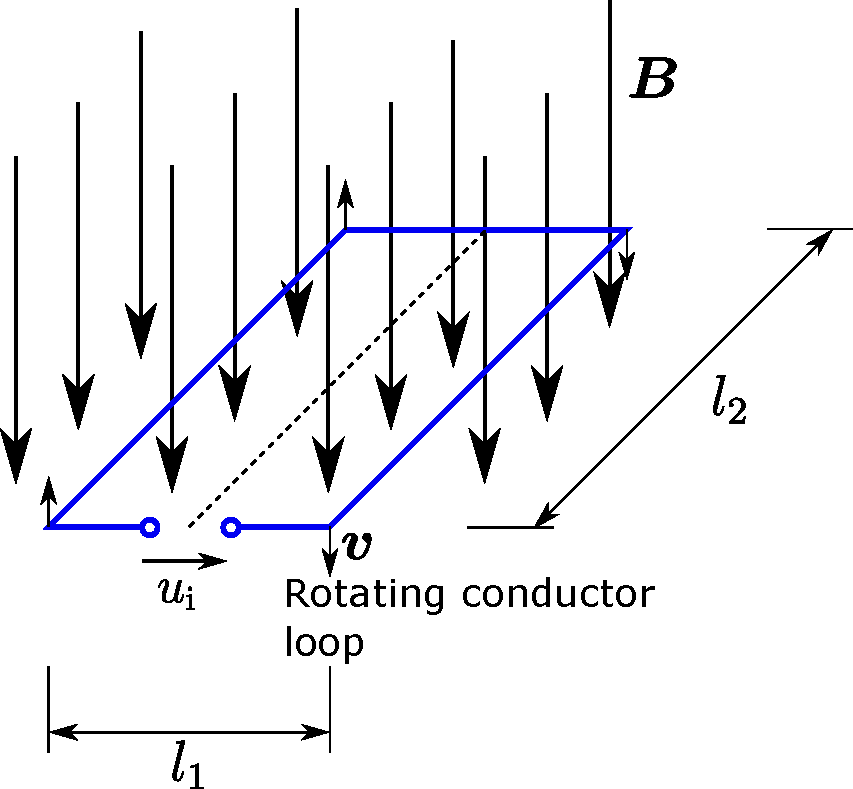
\includegraphics[height=0.6\textheight]{fig/lec02/Conductor_loop_induction.pdf}
				\caption{Induced voltage / EMF in a rotating conductor loop (adapted from: \href{https://commons.wikimedia.org/wiki/File:Leiterschleife.svg}{Wikimedia Commons}, M. Lenz, \href{https://creativecommons.org/publicdomain/zero/1.0/deed.en}{CC0 1.0})}
			\end{figure}
		\end{column}
		\end{columns}
\end{frame}

%%%%%%%%%%%%%%%%%%%%%%%%%%%%%%%%%%%%%%%%%%%%%%%%%%%%%%%%%%%%%
%% Intermediate wrap up: electromagnetic principles and magnetic materials (in inductive systems) %%
%%%%%%%%%%%%%%%%%%%%%%%%%%%%%%%%%%%%%%%%%%%%%%%%%%%%%%%%%%%%%
\begin{frame}
	\frametitle{Intermediate wrap up: electromagnetic principles and magnetic materials }
    \begin{figure}
        \centering
        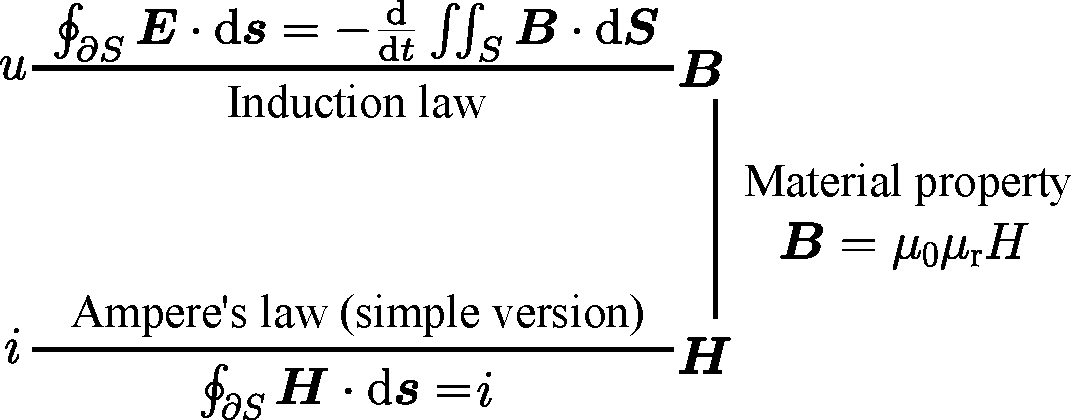
\includegraphics[height=0.5\textheight]{fig/lec02/Induction_material_ampere.pdf}
        \caption{Illustration of the connections between the phenomena discussed previously (derived from: \href{https://de.wikipedia.org/wiki/Datei:Kausalität.svg}{Wikimedia Commons}, M. Lenz, \href{https://creativecommons.org/publicdomain/zero/1.0/deed.de}{CC0 1.0})}
    \end{figure}
\end{frame}

%%%%%%%%%%%%%%%%%%%%%%%%%%%%%%%%%%%%%%%%%%%%%%%%%%%%%%%%%%%%%
%% Eddy currents %%
%%%%%%%%%%%%%%%%%%%%%%%%%%%%%%%%%%%%%%%%%%%%%%%%%%%%%%%%%%%%%
\begin{frame}
	\frametitle{Eddy currents}
    \begin{columns}
		\begin{column}{0.5\textwidth}
            \begin{itemize}
                \item  A changing magnetic field induces a voltage.
                \item In bulky conductive materials (e.g., electromagnetic steel) this voltage drives currents called eddy currents.
                \item Eddy currents lead to energy losses and heat dissipation.
                \item To reduce eddy currents, laminated cores are used as they decrease the effective current path width and, therefore, increase the effective resistance per sheet.
            \end{itemize}
		\end{column}
        \hfill
		\begin{column}{0.49\textwidth}
			\begin{figure}
				\centering
				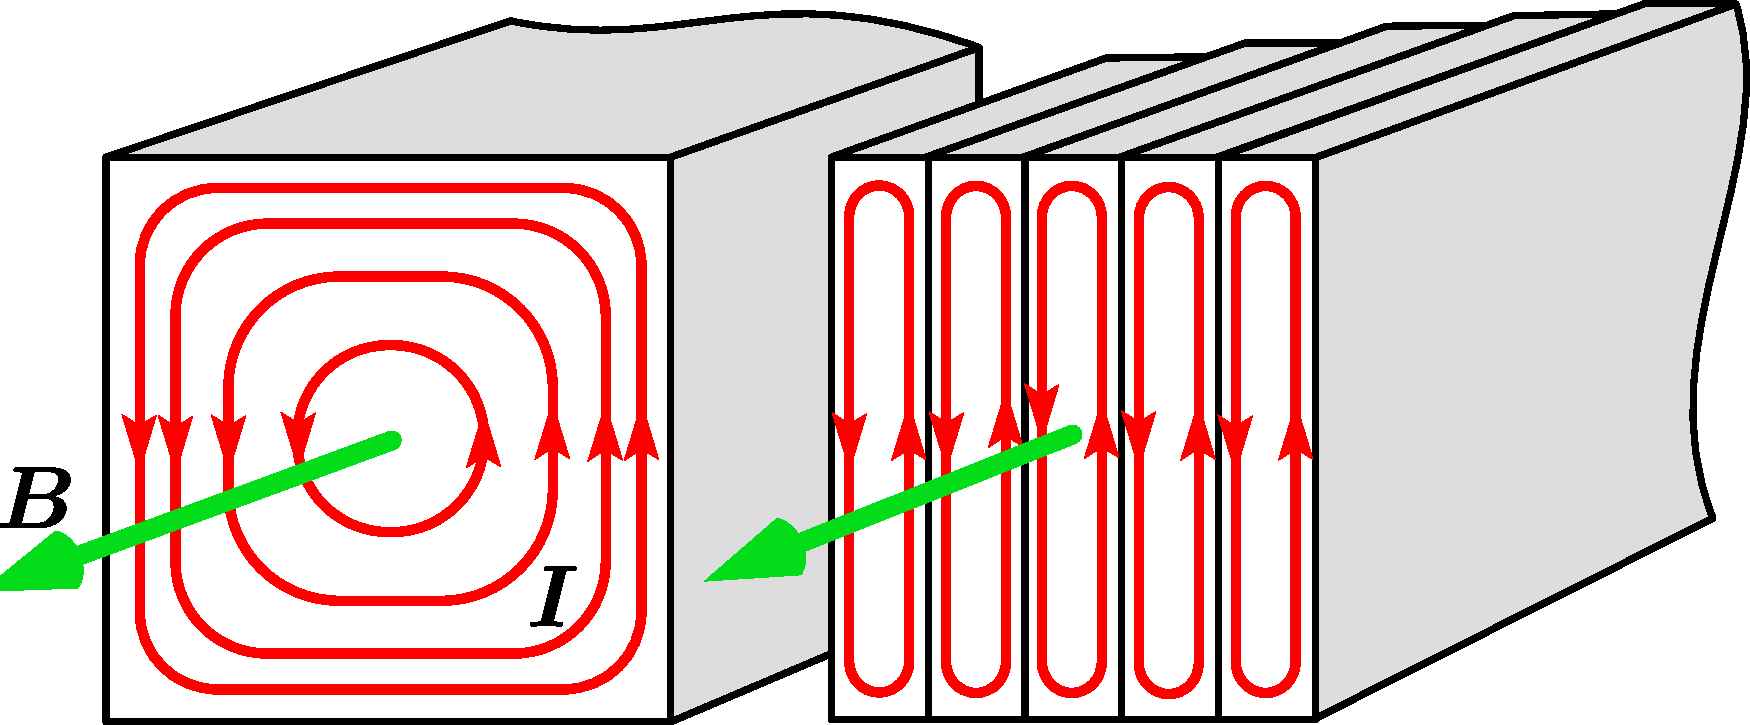
\includegraphics[height=0.36\textheight]{fig/lec02/Laminated_core_eddy_currents.pdf}
				\caption{Eddy current formations in solid and laminated steel cores (source: \href{https://commons.wikimedia.org/wiki/File:Laminated_core_eddy_currents.svg}{Wikimedia Commons}, Chetvorno, \href{https://creativecommons.org/publicdomain/zero/1.0/deed.en}{CC0})}
			\end{figure}
		\end{column}
		\end{columns}
\end{frame}